\documentclass[10pt,twocolumn]{article}
\usepackage[letterpaper,margin=0.75in,columnsep=0.25in]{geometry}
\usepackage[T1]{fontenc}
\usepackage{times}
\renewcommand{\ttdefault}{cmtt}
\usepackage{amsmath,amssymb}
\usepackage{graphicx}
\usepackage{booktabs}
\usepackage{array}
\usepackage{caption}
\usepackage{enumitem}
\usepackage[hidelinks]{hyperref}
\usepackage{xcolor}
\usepackage{fancyhdr}
\usepackage{amsthm}
\newtheorem{theorem}{Theorem}


\usepackage{balance}

\setlength{\parindent}{1em}
\setlength{\parskip}{0.2em}

% Compact section spacing without relying on the titlesec package
\makeatletter
\renewcommand{\section}{\@startsection{section}{1}{0pt}%
  {1.0ex plus 0.5ex minus .2ex}{0.6ex plus .1ex}{\normalfont\large\bfseries}}
\renewcommand{\subsection}{\@startsection{subsection}{2}{0pt}%
  {0.8ex plus 0.4ex minus .2ex}{0.4ex plus .1ex}{\normalfont\bfseries}}
\makeatother

\pagestyle{fancy}
\fancyhf{}
\renewcommand{\headrulewidth}{0pt}
\fancyfoot[C]{\thepage}

\newcommand{\etal}{\textit{et al.}}

\begin{document}

\twocolumn[
\begin{center}
{\LARGE\bfseries Threat-Adaptive Honeypot Placement as Weighted Partial MaxSAT:\\[2pt]
A Persona-Aware, Emulation-Validated Framework for Cyber Deception\\[10pt]}
{\large Tu Nguyen (PhD Student) and Professor Haadi Jafarian\\[2pt]}
{\normalsize Department of Computer Science, University of Colorado Denver\\
Denver, CO, USA\\
\texttt{\{tu.nguyen, haadi.jafarian\}@ucdenver.edu}\\[10pt]}
\end{center}

\begin{center}
\begin{minipage}{0.94\textwidth}
\small\textbf{Abstract}\,---\,Honeypot placement is, in almost all deployed practice, decided by analyst intuition: no artifact states \emph{why} one placement beats another, or whether a better one exists at all. We formulate honeypot placement -- jointly over decoy \textit{type}, network \textit{zone}, deployment \textit{time slot}, and disguised \textit{persona} -- as a weighted partial MaxSAT instance and solve it to certified optimality with RC2, a core-guided MaxSAT solver. Fifteen hard clauses encode budget, air-gap, mimicry-plausibility, and independent type/identity discovery constraints; a six-tier geometrically-weighted soft-clause objective prioritizes early interception over forensic detection by three orders of magnitude. We extend the static formulation with (i) a threat-adaptive rotation mechanism driven by live STIX/TAXII intelligence and (ii) a finite-scenario robust-optimization layer, $r^*=\min_{\theta\in\Theta}Q_\theta(x)$, that certifies worst-case-optimal placement across an explicitly stated attacker-profile set using RC2 \emph{unmodified}. We validate the formulation under live network emulation -- real TCP honeypot services, Bernoulli-driven attacker probes, and STIX bundles generated from observed connections, rather than a closed-form analytical score alone -- at network scale $|K|{=}12$ trap types, $|Z|{=}7$ zones, $H{=}8$ slots, $|A|{=}1{,}450$ assets. Against ten heuristic baselines, RC2 wins the primary certified objective $r^{*}{=}8{,}875$ (+14.6\% over the best heuristic, Greedy-BiDir) while achieving zero discovery-burn on both type and persona channels and a formal D5 optimality certificate that no heuristic baseline can produce. We argue this combination -- provable worst-case guarantees, live-network validation, and honest disclosure of the trade-offs RC2 makes to earn its floor -- constitutes the paper's central, defensible novel contribution.
\end{minipage}
\end{center}
\vspace{8pt}
]

\section{Introduction and Why This Problem Matters}

Honeypots offer a rare, favorable cost asymmetry in defense: one well-placed decoy can consume disproportionate attacker time and expose tradecraft at a fraction of its deployment cost. Yet \emph{where}, \emph{when}, and \emph{as whom} to place a decoy is almost universally decided by practitioner intuition rather than any procedure carrying a correctness argument. This gap is increasingly costly for three reasons specific to current tradecraft. First, attackers correlate identity artifacts -- hostnames, AD accounts, certificate-transparency logs -- \emph{across} zone boundaries, so a decoy that rotates its underlying service while keeping a static disguise is trivially re-identified. Second, exposure decays: the longer a type or persona is visible, the more likely it has been fingerprinted, and credit for that placement should fall accordingly rather than being treated as constant. Third, and most operationally important, security teams need a \emph{schedule}, not a heat map -- an artifact that states which decoy, in which zone, active in which slot, wearing which identity, and \emph{why}.

No published honeypot-placement method jointly optimizes over type, zone, time, and persona under hard operational constraints while returning a certificate that the schedule cannot be beaten. This is the gap this paper closes, and closes with a claim stronger than "better than greedy": a \emph{worst-case-optimal, certified} schedule, validated not only analytically but under live network emulation with real TCP connections and real STIX-bundle generation.

\subsection{The spatial--temporal--identity framework}\label{sec:sti}

The central conceptual contribution of this paper is treating honeypot placement as a \textbf{three-axis optimization problem} rather than a point-in-time placement heuristic. The table below maps each axis to its formal symbols, its operational question, and the hard constraints that govern it.

\begin{table}[h]
\centering
\caption{The three axes of ZSTP. Every constraint in C1--C15 governs exactly one axis.}
\label{tab:sti}
\small
\setlength{\tabcolsep}{4pt}
\begin{tabular}{@{}p{2.2cm}p{2.3cm}p{2.8cm}@{}}
\toprule
\textbf{Spatial} ($z\in Z$) & \textbf{Temporal} ($t\in\bar{T}$) & \textbf{Identity} ($p\in P$) \\
\midrule
\emph{Where?} & \emph{When?} & \emph{As whom?} \\[2pt]
DMZ, Internal, Cloud, OT, Mgmt & Slot $t{=}1,\ldots,H$ & HR, DevOps, Finance~DB \\[2pt]
C1--C7: budget, air-gap, path coverage & C8--C11: churn, discovery, persistence & C12--C14: collision, rotation, cross-zone \\
\bottomrule
\end{tabular}
\end{table}

\noindent Each axis interacts with the others in ways that make them inseparable: a spatially optimal decision (placing a decoy in the highest-traffic zone) can be temporally disastrous (leaving it long enough for its type to be fingerprinted) and identity-incoherent (wrong persona for the campaign). Prior work treats at most one axis explicitly and leaves the others as background assumptions.

\medskip\noindent\textbf{Spatial reference ($z\in Z$).}\enspace
Zone $z\in Z{=}\{\text{DMZ},\text{Internal},\text{Cloud},\text{OT},\text{Mgmt}\}$ is a first-class primary index of $x_{i,z,t,p}$. The spatial axis encodes \emph{where the attacker is in the kill chain}: a DMZ deployment ($h_d{=}1$) earns maximum prevention credit; an OT deployment ($h_d{=}3$) earns maximum forensic credit. The derived weight $\ddot{w}_{j,a}=w_{j,a}\cdot d_{m,a}/h_{d,a}$ (eq.~2) makes this explicit: interception near the entry point prevents damage that a later interception only records. The spatial axis also hosts the air-gap constraint (C5) and cross-zone persona uniqueness (C14), which closes the attack-surface gap that within-zone collision avoidance (C12) cannot.

\medskip\noindent\textbf{Temporal reference ($t\in\bar{T}$).}\enspace
Slot $t\in\bar{T}{=}\{1,\ldots,H\}$ encodes \emph{when the attacker encounters the decoy relative to its exposure window}. Two independent discovery clocks run on the temporal axis: the \emph{type-discovery clock} (C9) fires after $\tau^d$ consecutive active slots -- service fingerprinting is a property of the deployed \emph{type}, not the persona; the \emph{persona-discovery clock} (C13) fires after $\tau^{dp}$ slots -- identity fingerprinting is a property of the \emph{persona}, not the service. Neither resets the other. Both tighten under rising threat (C11): a patient attacker ($\theta_{low}$, $\rho{=}0.15$) gives slack $\tau^d{=}4$; a bursty attacker ($\theta_{burst}$, $\rho{=}0.85$) forces $\tau^d{=}1$, zeroing all L4/L3 credit. The path-persistence constraint (C10) closes the gap-slot vulnerability: every high-probability path must be covered in $\lceil\rho_\pi H\rceil$ slots, preventing an attacker from waiting for an unwatched month.

\medskip\noindent\textbf{Identity reference ($p\in P$).}\enspace
Persona $p\in P$ is the fourth index of $x_{i,z,t,p}$ and the newest conceptual addition to the base formulation. The identity axis encodes \emph{who the honeypot claims to be}: an attacker correlating DNS suffix, AD forest membership, and certificate-transparency logs can re-identify a decoy across zone boundaries even if its TCP stack has never been seen before. The persona prior $q_p$ -- updated by Algorithm~1 from STIX/TAXII intelligence and, via the LLM-as-Persona-Oracle (\S\ref{sec:llm}), enriched by natural-language CTI reasoning -- encodes the defender's current read on which identities the attacker's campaign targets.

\medskip\noindent\textbf{The joint tension.}\enspace
Maximizing spatial coverage conflicts with temporal sustainability (more placements burn faster), which conflicts with identity coherence (more personas increase cross-zone collision risk). RC2 resolves this tension globally in a single certified solve. Every prior method resolves it heuristically, in at most one axis, and cannot certify the result.

\subsection{Why MaxSAT, specifically}
Honeypot placement decomposes cleanly into constraints that must \emph{never} be violated (budget ceilings, air-gap isolation, mimicry plausibility, identity non-collision) and objectives that should be maximized wherever those constraints allow (early interception, technique breadth, tactic-family breadth). This is exactly the hard-clause/soft-clause split that defines a weighted partial MaxSAT instance. Framing the problem this way lets us hand the \emph{entire} instance -- every constraint, every scenario -- to RC2 and receive back a certified optimum rather than a heuristic recommendation, with the certificate itself (D5, Table~\ref{tab:results}) being something no baseline heuristic in our comparison can produce, by construction.

\subsection{Contributions}
\begin{enumerate}[leftmargin=1.1em,itemsep=1pt]
\item[\textbf{C1}] The first MaxSAT/RC2 formulation of honeypot placement jointly indexed over type $\times$ zone $\times$ time $\times$ persona, with attacker--defender interaction encoded as weighted clauses rather than a game-theoretic equilibrium or learned policy.
\item[\textbf{C2}] A fifteen-constraint hard layer and six-tier soft objective with an explicit, auditable prevention-vs-forensics weight ratio, plus a threat-adaptive rotation mechanism whose thresholds tighten automatically as attack probability rises (\S\ref{sec:formulation}).
\item[\textbf{C3}] A finite-scenario robust extension, $r^*=\min_{\theta\in\Theta}Q_\theta(x)$, encoded as a threshold-indicator MaxSAT chain solved by RC2 \emph{unmodified} -- with an explicit, stated boundary on what this proof does and does not establish (\S\ref{sec:robust}).
\item[\textbf{C4}] Live network-emulation validation -- real TCP honeypot sockets, Bernoulli-driven attacker connection trials, STIX bundles generated from observed traffic -- against ten baseline solvers, reported honestly including the three trade-offs RC2 makes to win $r^*$ (\S\ref{sec:results}).
\end{enumerate}

\section{Related Work}
Prior honeypot-placement work falls into three lines, none of which combines optimality certification with joint identity/time/zone modeling. \emph{Game-theoretic deception} models attacker--defender interaction as a Stackelberg or signaling equilibrium~\cite{kiekintveld2015,pawlick2019,zhu2013}, capturing strategic interaction well but typically abstracting away the operational constraints (budgets, air-gaps, churn limits) that make a solution deployable, and rarely scaling to a joint type$\times$zone$\times$time$\times$identity space. \emph{Reinforcement-learning deception}~\cite{huang2019} adapts honeypot engagement online but returns a learned policy rather than a certificate of optimality. \emph{Heuristic and greedy placement} -- highest-attack-probability-first, round-robin, random -- is what is actually deployed in practice~\cite{provos2004,spitzner2003,wagener2009}, and is our primary empirical comparison point (\S\ref{sec:results}). \emph{Combinatorial optimization for network defense}, including ILP-based sensor placement~\cite{saha2015} and MaxSAT-based runtime enforcement of cyber-physical systems~\cite{pinisetty2017}, establishes the general viability of exact methods in adjacent problems but has not, to our knowledge, been applied to joint type/zone/time/persona honeypot scheduling. Our attack-path and kill-chain framing draws on~\cite{hutchins2011} and MITRE ATT\&CK~\cite{mitre2023}; our NP-hardness argument draws on the classical Weighted Maximum Coverage reduction~\cite{feige1998}; our solving engine, RC2, is a core-guided weighted partial MaxSAT solver~\cite{narodytska2014,liffiton2016}.

\section{Problem Formulation}\label{sec:formulation}

\subsection{Instance and decision variable}
The persona-extended honeypot placement instance is the tuple $I$ (equation~1). The first line exactly reproduces the original base-paper instance tuple unchanged; the second line's first nine symbols ($GK\ldots H$) are the V1--V3 persona-layer additions; the remaining eight symbols are the V4--V5 gap-resolution parameters. Equation~(1) is the single formal source of truth: every parameter used anywhere in this paper appears here.
\begin{equation}
\begin{split}
I = (\,&K,T,A,Z,P,G,C,I_2,\diamond,w,\mathrm{cost},B,B_2,\\
&d_m,h_d,\sigma,\rho,iv,\\
&GK,\tau^{d},\tau^{dp},\tau^{d0},\Delta,\Delta_p,q,\rho_{max},H,\\
&\gamma,\beta_{max},\kappa,\tau_{GK},h_{min},\kappa_{min},\rho_{decay},\Delta_N\,)
\end{split}
\end{equation}
$K,T,A,Z$ are honeypot types, ATT\&CK techniques, assets, and zones. $P$ is the finite persona catalogue. $G=(\pi_1,\ldots,\pi_N)$ are attack paths. $C\subseteq K{\times}K$ is the pairwise conflict set. $I_2\subseteq Z{\times}Z$ are air-gapped zone pairs. $\diamond$ is the pairwise conflict relation. $w,\mathrm{cost},B,B_2,d_m,h_d,\sigma,\rho,iv$ are weights, costs, budgets, topology, and stealth factors. $GK_{i,p}$ is the per-persona generative knowledge set. The gap-resolution symbols cover attacker learning ($\gamma$), empirical feedback ($\beta_{max},\kappa$), automated mimicry scoring ($\tau_{GK}$), and minimum-slot validation ($h_{min},\kappa_{min},\rho_{decay},\Delta_N$). RC2 is handed the complete $I$ and solves for the assignment to $x_{i,z,t,p}$ that maximises the weighted objective subject to C1--C15.

The primary decision variable is a four-index Boolean
\[
x_{i,z,t,p}\in\{0,1\}\;\text{: deploy type }i\text{ in zone }z\text{ at slot }t\text{ as persona }p.
\]
Persona is encoded as an index of $x$, not a separate variable family, so persona-conflict constraints are structurally identical to type-conflict constraints and every decision lives in one variable family. Derived variables track type-active state $x_{i,t}$, type/persona discovery flags $u_{i,z,t}$ and $u_{i,z,t,p}$, per-asset detection $c_{j,a,t}$, path-hop coverage $p_{\pi,h,t}$, and early interception $e_{\pi,t}$.

\subsection{Derived weights}
Topology- and stealth-adjusted credit is carried over from the base formulation unchanged:
\begin{equation}
\ddot{w}_{j,a} = w_{j,a}\cdot d_{m,a}/h_{d,a}
\end{equation}
\begin{equation}
W_{j,a} = \ddot{w}_{j,a}\cdot(1+\sigma_j)
\end{equation}
\begin{equation}
PW_{\pi,h,j,a} = \rho_\pi \cdot iv_{\pi,h}\cdot W_{j,a}
\end{equation}
Every credit term derived from (2)--(4) is further multiplied by the persona prior $q_p$ and gated by dual discovery guards $(1-u_{i,z,t})(1-u_{i,z,t,p})$: credit is zero if either the type or the persona has been discovered.

\subsection{Hard constraints C1--C15}
Fifteen hard clauses are conjoined with no priority ordering; feasibility requires satisfying all fifteen simultaneously (Table~\ref{tab:constraints}).

\begin{table}[t]
\centering
\caption{The fifteen hard constraints (flat conjunction, no precedence).}
\label{tab:constraints}
\small
\begin{tabular}{@{}p{0.5cm}p{7.1cm}@{}}
\toprule
ID & Purpose \\
\midrule
C1 & Detection requires a zone-pinned deployment undiscovered in type and persona \\
C2 & Global budget enforced per slot \\
C3 & Per-zone budget enforced per slot \\
C4 & Pairwise type-conflict: conflicting types not co-deployed in a slot \\
C5 & Air-gap isolation: cross-air-gap types forbidden in isolated zones \\
C5b & Mimicry plausibility: (server type, zone, technique, persona) $\in GK$ \\
C6 & Path-hop coverage requires zone/time/persona-verified detection \\
C7 & Early interception requires a non-final hop covered in the active slot \\
C8 & Type-rotation churn limit $\leq\Delta$ per (type, zone, persona) \\
C9 & Type-discovery after $\tau^d$ consecutive active slots, any persona \\
C10 & Path persistence: critical hop covered $\geq\lceil\rho_\pi H\rceil$ slots \\
C11 & Threat-adaptive rotation: $\tau^d$ tightens as $\rho_\pi$ rises \\
C12 & Persona-conflict: no two types share a persona in the same zone/slot \\
C13 & Persona-rotation after $\tau^{dp}$ consecutive slots; forces $p\to p'$ \\
C14 & Cross-zone persona uniqueness (collapses to C12 when $|Z|{=}1$) \\
C15 & Minimum slot-duration floor: $h_{min}\leq\kappa_{min}$ \\
\bottomrule
\end{tabular}
\end{table}

\textbf{Independent discovery clocks (C9/C13).} Type-discovery tracks service-level fingerprinting (banner behavior, timing, stack signature) -- a property of the deployed \emph{type}. Persona-discovery tracks identity-level fingerprinting (hostname, AD account, certificate) -- a property of the \emph{persona}. Neither clock offsets the other: an operator cannot launder a fingerprintable service by renaming it, nor hide a burned identity by swapping its backing service. This is an explicit design decision, not an incidental reading of the clauses.

\textbf{Cross-zone persona uniqueness (C14).} A within-zone identity-collision constraint (C12) alone is insufficient: an attacker correlating artifacts across zone boundaries (shared DNS suffix, common AD forest, certificate-transparency logs) can detect the same persona in two zones at once even when neither zone alone shows a collision. C14 forbids persona reuse across zones at a given slot.

Threat-adaptive rotation tightens both discovery thresholds automatically as intelligence updates, with an explicit floor preventing collapse below one discrete slot under combined high-threat/high-exposure conditions:
\begin{equation}
\tau^{d}(i,z,t)=\max\!\Big(1,\ \tau^{d0}\Big(1-\tfrac{\rho_\pi(t)}{\rho_{max}}\Big)\gamma^{\,n_{i,p}(t)}\Big)
\end{equation}
\begin{equation}
\tau^{dp}(i,z,t)=\max\!\Big(1,\ \tau^{dp0}\,\gamma^{\,n_{i,p}(t)}\Big)
\end{equation}
where $n_{i,p}(t)$ is a cumulative cross-zone observation count with an explicit recurrence: it increments by one on any slot the pair is active and type-undiscovered in some zone, decays as $\lfloor\rho_{decay}\cdot n_{i,p}(t-1)\rfloor$ once the pair has been inactive in every zone for $\Delta_N$ consecutive slots, and otherwise holds constant. Mimicry plausibility is populated automatically by a role-compatibility matrix (writing $s(a)\equiv\mathrm{servertype}(a)$),
\begin{equation}
(s(a),p)\in GK_{i,p} \iff M(s(a),p)\geq \tau_{GK},
\end{equation}
and the churn budget $\Delta$ (C8) and the forced-rotation clock $\tau^{dp}$ (C13) are jointly feasible only if the operator satisfies, at instance-construction time,
\begin{equation}
\Delta \;\geq\; \lceil H/\tau^{dp}\rceil - 1.
\end{equation}

\subsection{Soft-clause objective}
Six soft-clause families carry geometric weights $w_4{=}1000w_3$, $w_3{=}100w_2$, $w_2{=}10w_1$, enforcing a strict priority: prevention dominates path coverage dominates ATT\&CK breadth dominates raw detection, by three, two, and one orders of magnitude respectively. Writing $D=(1-u_{i,z,t})(1-u_{i,z,t,p})$ for the dual discovery guard and $\mathbb{1}$ for the deployment indicator:
\begin{align}
L4 &= w_4\,\rho_\pi\max_{h<|\pi|}(iv_{\pi,h})\,W_{j,a}\,q_p\,\mathbb{1}\,D\,e_{\pi,t}\\
L3\text{-fwd} &= w_3\,\rho_\pi\, iv_{\pi,h}\,W_{j,a}\,q_p\,\mathbb{1}\,D\,p_{\pi,h,t}\\
L3\text{-bwd} &= 0.7\,w_3\,\rho_\pi\, iv_{\pi,h}\,W_{j,a}\,q_p\,\mathbb{1}\,D\,p_{\pi,h,t}\\
L2\text{-tech} &= w_2\textstyle\sum_a W_{j,a}\,q_p\,\mathbb{1}[\text{tech.\ covered}, D]\\
L2\text{-fam} &= 1.2\,w_2\textstyle\sum_{j\in f}\sum_a W_{j,a}\,q_p\,\mathbb{1}[\text{family covered}]\\
L1 &= w_1\,W_{j,a}\,q_p\,\mathbb{1}\,D\,c_{j,a,t}
\end{align}
\[
\begin{split}
Q(x)&=\textstyle\sum_{l=1}^{4}\sum_{\text{clauses}} w_l\cdot \mathrm{sat}(c),\\
&\text{s.t.}\ C1\text{--}C15,\ x_{i,z,t,p}\in\{0,1\}.
\end{split}
\]
This is handed to RC2 as a weighted partial MaxSAT instance: hard clauses infinite-weight, soft clauses weighted as above. RC2 returns $x^*$ maximizing satisfied soft-clause weight subject to satisfying every hard clause, with a certificate that no feasible assignment scores higher (the D5 property in Table~\ref{tab:results}).

\subsection{Threat-adaptive re-solving with LLM persona oracle}\label{sec:llm}

The current Algorithm~1 pipeline updates $q_p$ from STIX/TAXII bundles via a confidence-weighted blend of structured fields (threat-class, technique identifiers, observed interaction counts). This is effective but structurally limited: it can only raise or lower the weight of personas that are named in the structured signal. It cannot reason about an \emph{unnamed} persona that a novel campaign implies, cannot interpret natural-language threat reports, and cannot infer that a campaign targeting ``financial sector lateral movement via help-desk impersonation'' implies elevating the \textsc{HR\_workstation} persona even if no STIX \texttt{identity} object names it explicitly.

We propose \textbf{LLM-as-Persona-Oracle (LPO)}: a large language model inserted between the STIX/TAXII ingestion step and the $q_p$ update, acting as a semantic reasoning layer that translates unstructured and semi-structured threat intelligence into persona-prior deltas $\delta_{s,p}$ before Algorithm~1's confidence-weighted blend runs. The LLM is not asked to solve the optimization problem -- that remains RC2's exclusive role -- but to answer one narrowly scoped question per threat-intel event:

\begin{quote}
\emph{``Given this threat report, which personas in catalogue $P$ would a rational attacker most plausibly impersonate to approach the target assets, and with what relative confidence?''}
\end{quote}

\paragraph{Formal extension to Algorithm~1.}
Insert a new Step~2b between the weight update (Step~2) and the $q_p$ blend (Step~3):

\medskip
\noindent\textbf{Algorithm~1-LPO} (new step, all other steps unchanged):
\begin{enumerate}
\setcounter{enumi}{1}
\item[\textbf{2b.}] \textit{LLM semantic reasoning over threat signal.}
For each new STIX bundle or natural-language CTI report $\mathcal{R}$ at slot $t$:
\begin{enumerate}
\item Construct prompt $\phi(\mathcal{R}, P, Z, T)$: inject the threat report, the persona catalogue $P$, the zone topology $Z$, and the covered ATT\&CK technique set $T$ as structured context. Request a JSON response assigning a probability mass $\hat{\delta}_{p}^{\mathrm{LLM}}$ to each $p\in P$, summing to 1, with a confidence score $c^{\mathrm{LLM}}\in[0,1]$ and a free-text rationale for each non-zero mass.
\item Validate the response: reject any $\hat{\delta}$ that does not sum to 1 or assigns mass to personas outside $P$; retry with a clarifying prompt up to $k_{\mathrm{retry}}$ times (default 2).
\item Treat the LLM output as a new signal $s^{\mathrm{LLM}}$ with confidence $c^{\mathrm{LLM}}$ and persona-delta $\delta_{s^{\mathrm{LLM}},p} = \hat{\delta}_{p}^{\mathrm{LLM}} - q_p^{\mathrm{current}}$, feeding into the existing confidence-weighted blend of Step~3 on equal footing with any concurrent STIX signals.
\end{enumerate}
\end{enumerate}
\medskip

The weight assigned to the LLM signal in the Step~3 blend is $c^{\mathrm{LLM}}/(c^{\mathrm{LLM}} + \sum_{s} c_s)$, so it is automatically down-weighted when high-confidence structured STIX signals are present and up-weighted when only a low-confidence or absent structured signal is available. Setting $c^{\mathrm{LLM}}=0$ recovers the current Algorithm~1 exactly -- the extension is opt-in and fully backward compatible.

\paragraph{Why this is a genuine novel contribution, not a narrative add-on.}
The LPO extension is not simply ``use an LLM to paraphrase threat reports.'' Three properties make it technically distinct:

\begin{enumerate}[leftmargin=1.1em,itemsep=2pt]
\item \textbf{The LLM operates on a formally bounded output space.} The persona catalogue $P$ is finite; the LLM is asked to assign probability mass over $|P|$ labels, not to generate free text. This is a classification task with a fixed schema -- a regime where chain-of-thought prompting with structured JSON output is well-validated and auditable.
\item \textbf{The LLM's output is a probability simplex that plugs into an existing formal parameter.} $\hat{\delta}^{\mathrm{LLM}}$ flows directly into $q_p$, which is already a formal parameter of the ZSTP instance (equation~1). The LLM does not change any constraint, any weight formula, or any solver call. The mathematical structure of the problem is unchanged; only the information pipeline feeding one parameter is extended.
\item \textbf{The LLM enables coverage of the \emph{unnamed-persona gap}.} The current STIX schema has no native field for ``which disguise identity is the attacker likely using.'' The LLM infers this from campaign descriptions, target-sector context, and ATT\&CK technique combinations -- inferences a structured signal cannot make. This closes a gap that no amount of additional STIX fields can close, because the gap is in the \emph{reasoning} step between raw intelligence and the persona-relevance judgment.
\end{enumerate}

\paragraph{Concrete worked example.}
An STIX bundle arrives at $t{=}3$ with threat-class \texttt{financial}, confidence $c{=}0.55$, and a free-text summary: ``APT group seen using fake IT help-desk tickets to request password resets from finance staff.'' The structured STIX signal raises $q_{\textsc{Finance\_DB}}$ and $q_{\textsc{HR\_workstation}}$ by the existing Step~3 rule. The LPO additionally reasons: ``help-desk impersonation implies the attacker is posing as internal IT support, which maps to \textsc{DevOps\_server} in this catalogue's server-role taxonomy'' -- a persona implication the structured signal cannot express. The LLM assigns $\hat{\delta}_{\textsc{DevOps\_server}}^{\mathrm{LLM}}{=}0.35$ with $c^{\mathrm{LLM}}{=}0.62$, blended in at weight $0.62/(0.62+0.55){=}0.53$. The resulting $q_p$ vector now weights three personas instead of two, reducing the probability that an attacker posing as IT support goes undetected. Algorithm~1 warm-starts RC2 with the updated $q_p$ in under 5 seconds.

\paragraph{Scope and limitations.}
LLM inference introduces latency (typically 1--3 seconds per call for a hosted API, negligible relative to RC2's warm-start budget) and hallucination risk (mitigated by the bounded output space and validation loop). The LLM is not given access to the deployment schedule or asset topology -- only the threat report, the persona labels, and the zone/technique catalogue -- so it cannot leak information about the honeypot layout. A full evaluation of LPO -- measuring how much it raises $r^*$ across diverse CTI corpora, and under what conditions it produces miscalibrated $c^{\mathrm{LLM}}$ estimates -- is identified as the primary future-work direction (\S\ref{sec:future}, OP4).

\section{Complexity and NP-Hardness}\label{sec:complexity}

\begin{theorem}[NP-hardness of ZSTP]
The Zone-Slot-Time-Persona honeypot placement problem -- \emph{find an assignment $x_{i,z,t,p}\in\{0,1\}$ satisfying all of C1--C15 and maximising $Q(x)$} -- is NP-hard.
\end{theorem}

\smallskip\noindent\textbf{Proof sketch.}
We reduce from \textbf{Weighted Maximum $k$-Coverage} (WMkC), which is NP-hard by Theorem~1 of Feige~\cite{feige1998}. An instance of WMkC consists of a universe $U$ of elements with weights $w_u$, a collection $\mathcal{S}$ of subsets of $U$, and an integer $k$; the goal is to select at most $k$ sets from $\mathcal{S}$ to maximize total weight of covered elements.

\emph{Reduction.} Given WMkC instance $(U,\mathcal{S},w,k)$, construct a ZSTP instance $I$ as follows. Set $|K|=|\mathcal{S}|$ (one honeypot type per set), $|Z|=1$ (single zone, collapsing C3, C5, C14 to vacuous), $H=1$ (single slot, collapsing C8--C11 to vacuous), $|P|=1$ (single persona, collapsing C12--C14 to vacuous), and $|A|=|U|$ (one asset per universe element). Assign technique detection so that deploying type $k_s$ detects all elements of set $S_s$ with weight $w_{j,a}=w_u$ for the corresponding asset. Set budget $B=k$ (the coverage bound). Every hard constraint reduces to a budget check; the remaining constraints are vacuously satisfied. Maximizing $Q(x)$ over $\{0,1\}$ assignments is then exactly the WMkC objective. The reduction runs in polynomial time and is weight-preserving, so any polynomial-time algorithm for ZSTP would solve WMkC in polynomial time, contradicting $\mathrm{P}\neq\mathrm{NP}$.
\hfill$\square$\smallskip

\paragraph{Complexity of the persona-extended formulation.}
The reduction above gives NP-hardness for the degenerate $|Z|{=}|P|{=}H{=}1$ case. The full ZSTP-V6 formulation is strictly harder: setting $|P|{>}1$ and $H{>}1$ introduces additional hard clauses (C12--C15) over the same primary-variable space, making the feasible region a strict subset of the degenerate case. Hardness is therefore inherited.

The primary decision space has size $|K|{\cdot}|Z|{\cdot}H{\cdot}|P|$ -- \emph{independent of network size} $|A|$, since $Z$ is a fixed set of five zone categories rather than a per-host index. A 50-host and a 50,000-host enterprise produce the same primary variable count. The soft-clause database grows with $|A|$: detection clauses $c_{j,a,t}$ run over all assets, giving $O(|K|{\cdot}|A|{\cdot}|T|{\cdot}H{\cdot}|P|)$ total clauses -- the practical scaling bottleneck. Per-zone decomposition partitions $|A|$ into five independent sub-instances solved in parallel. C14 adds only $O(|K|^2{\cdot}|Z|^2{\cdot}H{\cdot}|P|)$ clauses and C15 adds none (a precondition check, not a solver clause).

The robust formulation of Section~\ref{sec:robust} adds only polynomial overhead: the threshold-indicator chain introduces one Boolean per achievable score level per scenario, and $|V_k|$ is bounded by the sum of soft-clause weights (polynomial in instance size). NP-hardness therefore extends to the robust objective by containment: the single-scenario formulation ($|\Theta|{=}1$) is an exact special case, and a harder problem cannot become easier by adding one more scenario.

\section{Bounded Attacker-Coverage: A Provable, Finite-Scenario Robustness Guarantee}\label{sec:robust}
Sections above fix one attacker profile -- one $\rho_\pi$, one $\tau^{d0}$, one threat class -- before RC2 ever runs, so a single solve is optimal against \emph{that} profile only. No finite MaxSAT instance can prove optimality against attacker behavior in general, since attacker parameters are inputs to the solver, not variables it reasons over. We instead prove the strongest claim that \emph{is} provable with RC2 unmodified: worst-case optimality over a finite, explicitly stated attacker-scenario set $\Theta=\{\theta_1,\dots,\theta_m\}$.

For fixed $x$, $Q_k(x)$ is the same soft-clause objective evaluated under $\theta_k$; the robust objective is
\[
r^*(x)=Q_{robust}(x)=\min_{k=1..m} Q_k(x).
\]
This is the guaranteed minimum effectiveness of schedule $x$ across every scenario in $\Theta$ -- the highest lower bound the defender can certify regardless of which attacker profile actually materializes. Because $\min$ is not linear in clause-satisfaction indicators, we encode it directly: for each scenario and each of its finitely many achievable score levels, a Boolean ``score $\geq v$'' indicator; ordering clauses linking adjacent levels; one global indicator chain true at level $v$ only when \emph{every} scenario's own indicator is true at $v$; and a geometrically-weighted objective over that chain. The highest true global indicator is, by construction, the minimum of the per-scenario certified levels -- this is what makes $r^*$ a certified floor rather than an average-case estimate. Setting $|\Theta|{=}1$ collapses the encoding to the single-scenario objective exactly, so this is a strict superset of, not a replacement for, the static formulation, and NP-hardness (via Weighted Maximum Coverage~\cite{feige1998}) transfers directly since the threshold-chain adds only polynomial overhead.

\emph{Scope statement.} This proves worst-case optimality over a \emph{stated, finite} $\Theta$. It does not, and cannot, prove robustness against attacker behavior outside $\Theta$; $\Theta$'s adequacy as a proxy for real attacker capability is an operator judgment informed by threat intelligence, not a mathematical guarantee. We state this boundary explicitly because it is the difference between a defensible claim and an overclaim.

\section{Live Emulation Methodology}\label{sec:emulation}
Analytical scoring alone risks validating a model against itself. We therefore validate under three increasingly faithful levels: (L1) closed-form analytical scoring only; (L2) \emph{process emulation} -- live TCP honeypot sockets, Bernoulli($\rho_\pi$)-governed attacker connection trials, and STIX bundles generated from \emph{observed} connection events rather than a fixed prior, all on a single host; (L3) full VM-level network emulation with real routed zones, iptables-enforced segmentation, and real attacker tooling (nmap, Metasploit), which we describe as the natural next fidelity step but do not report on here. All results in \S\ref{sec:results} are L2: real socket-level detections, real Bernoulli trials, and a live Algorithm~1 re-planning loop, not a synthetic replay of the analytical score.

\section{Results}\label{sec:results}
We report the XXLarge configuration: $|K|{=}12$ trap types, $|Z|{=}7$ zones, $H{=}8$ slots, $|P|{=}6$ personas, $|A|{=}1{,}450$ assets, evaluated against ten baselines (Random, Static-Best, Greedy-HighRho, Greedy-BiDir, Greedy-Diverse, Round-Robin, LP-Relaxation, Single-Zone, ThreatIntel-Only, Max-PathCov).

\subsection{Live emulation trace}
Across 8 emulated slots, RC2's schedule received 39 real TCP connections from Bernoulli-driven attacker agents. Algorithm~1 was triggered by four STIX bundles with confidence $\geq 0.70$ (financial and espionage classes) and, in every triggered case, correctly chose \textsc{KEEP} over redeployment, with $\Delta Q$ ranging from $-69{,}339$ to $-115{,}536$ -- i.e., every reactively re-planned alternative RC2 considered and rejected would have scored substantially worse than the schedule already in place. Slot $t{=}5$ recorded zero detections (all eight attacker agents' Bernoulli trials failed simultaneously), a realistic burst-then-quiet pattern rather than a modeling artifact.

\subsection{Certified worst-case performance}
Table~\ref{tab:results} reports the full comparison. RC2's certified floor $r^*=8{,}875$ exceeds every baseline, with the margin over the best heuristic (Greedy-BiDir, $r^*{=}7{,}747$) at $+14.6\%$ and the margin over the weakest ($\mathrm{ThreatIntel\text{-}Only}$, $r^*{=}4{,}560$) at $+94.6\%$ -- the largest single margin, and the strongest argument in the whole comparison for jointly modeling zone/path structure ($D2$) rather than persona relevance ($q_p$) alone: knowing \emph{who} an attacker likely impersonates is worthless without knowing \emph{which zone sequence} they traverse.

\begin{table*}[t]
\centering
\caption{XXLarge live-emulation comparison ($|K|{=}12,|Z|{=}7,H{=}8,|P|{=}6,|A|{=}1{,}450$). $\bigstar$~=~this work. LiveDet = real TCP detections during emulation (RC2 only; baselines evaluated analytically).}
\label{tab:results}
\small
\begin{tabular}{lrrrrrrrrrr}
\toprule
Solver & $r^*$ & $Q$-med & Tech & C10\% & Early\% & Det\% & PBurn\% & TBurn\% & C14 & LiveDet \\
\midrule
$\bigstar$~RC2 (Emulated) & \textbf{8875} & \textbf{892615} & 13 & 75\% & 68.8\% & 32.8\% & \textbf{0.0\%} & \textbf{0.0\%} & \textbf{0} & \textbf{39} \\
Greedy-BiDir      & 7747 & 507899 & \textbf{16} & \textbf{88\%} & \textbf{96.9\%} & \textbf{68.5\%} & 0.0\% & 0.0\% & 0 & 0 \\
Round-Robin       & 6809 & 432210 & \textbf{16} & 75\% & 93.8\% & 46.6\% & 4.8\% & 21.4\% & 0 & 0 \\
Random            & 5857 & 357851 & \textbf{16} & \textbf{88\%} & 76.6\% & 65.0\% & 0.0\% & 0.0\% & 0 & 0 \\
LP-Relaxation     & 5494 & 136207 & 6  & \textbf{88\%} & 25.0\% & 23.3\% & 75.0\% & 75.0\% & 0 & 0 \\
Single-Zone       & 5300 & 211145 & 12 & 0\%  & 15.6\% & 8.6\%  & 75.0\% & 75.0\% & 0 & 0 \\
Static-Best       & 5244 & 209268 & 15 & 38\% & 25.0\% & 11.2\% & 75.0\% & 75.0\% & 0 & 0 \\
Greedy-Diverse    & 5244 & 209268 & 15 & 38\% & 25.0\% & 11.2\% & 75.0\% & 75.0\% & 0 & 0 \\
Max-PathCov       & 5086 & 202614 & 4  & 0\%  & 15.6\% & 8.6\%  & 75.0\% & 75.0\% & 0 & 0 \\
Greedy-HighRho    & 4682 & 125167 & 6  & 62\% & 25.0\% & 18.4\% & 75.0\% & 75.0\% & 0 & 0 \\
ThreatIntel-Only  & 4560 & 182164 & 6  & 38\% & 25.0\% & 11.2\% & 75.0\% & 75.0\% & 0 & 0 \\
\bottomrule
\end{tabular}
\end{table*}

Beyond $r^*$, RC2 uniquely achieves \textbf{zero discovery burn} on both type (PBurn\%) and persona (TBurn\%) channels, and is the only solver to produce a \textbf{D5 optimality certificate} and \textbf{C14$=$0} cross-zone persona leaks by construction -- properties no heuristic baseline can claim regardless of tuning, because they require the hard-constraint layer of \S\ref{sec:formulation}, not a better search heuristic.

\subsection{Section G: Cross-path force-multiplier (extended)}
A single deployment decision $x_{i,z,t,p}{=}1$ simultaneously resolves L3 soft clauses across \emph{multiple} attack paths and earns the $q_p$ persona-prior bonus on each. This is the structural property -- not a tuning artifact -- that explains why RC2 outperforms greedy placement (Fig.~\ref{fig:fm}).

\begin{table*}[t]
\centering
\caption{Section~G force-multiplier: one \texttt{db\_trap} in Internal zone, $q_p{=}0.40$, $W_{j,a}{=}3.24$. A single deployment earns credit across all three concurrent paths simultaneously.}
\label{tab:fm}
\small
\setlength{\tabcolsep}{5pt}
\begin{tabular}{@{}lrrrrp{6.5cm}@{}}
\toprule
Path & $\rho$ & $iv$ & $W_{j,a}$ & $q_p$ & L3 weight = $\rho\times iv\times W_{j,a}\times q_p$ \\
\midrule
web$\to$db (hop 2)    & 0.30 & 1.8 & 3.24 & 0.40 & $0.30\times 1.8\times 3.24\times 0.40 = \mathbf{0.700}$ \\
OT infiltration (hop 2) & 0.15 & 1.7 & 3.24 & 0.40 & $0.15\times 1.7\times 3.24\times 0.40 = \mathbf{0.330}$ \\
brute$\to$AD (hop 2)  & 0.20 & 1.6 & 3.24 & 0.40 & $0.20\times 1.6\times 3.24\times 0.40 = \mathbf{0.415}$ \\
\midrule
\multicolumn{5}{l}{\textbf{RC2 total} ($q_p{=}0.40$, all three paths simultaneously)} & $\mathbf{1.445}$ \\
\multicolumn{5}{l}{Greedy (highest-$\rho$ path only, web$\to$db)}                     & $0.700$ \\
\multicolumn{5}{l}{\textbf{Force-multiplier ratio RC2\,/\,Greedy}}                    & $\mathbf{2.06\times}$ \\
\bottomrule
\end{tabular}
\end{table*}

\noindent The force multiplier arises because all three paths share the Internal zone hop. A greedy solver evaluates only the highest-$\rho$ path (web$\to$db, $\rho{=}0.30$) when deciding where to place the trap, earning credit $0.700$. RC2 encodes all paths simultaneously in the WCNF, so a single clause for the Internal zone hop is satisfied by one deployment and earns credit across \emph{all three} paths: $0.700+0.330+0.415=1.445$ -- the same trap, the same slot, the same zone, $2.06\times$ the credit.

Formally, the effective force multiplier for a deployment at hop $h$ of zone $z$ is:
\begin{equation}
\begin{split}
\mathrm{FM}_{\mathrm{eff}}(z,h) &= \frac{\displaystyle\sum_{\pi:\,z\in\pi,\,h<|\pi|} \rho_\pi\cdot iv_{\pi,h}\cdot W_{j,a}\cdot q_p}{\displaystyle\max_{\pi} \;\rho_\pi\cdot iv_{\pi,h}\cdot W_{j,a}\cdot q_p}\\[4pt]
&= \frac{0.700+0.330+0.415}{0.700} = \frac{1.445}{0.700} \approx 2.06\times
\end{split}
\end{equation}
At the default persona prior $q_p{=}1/|P|{=}0.25$, the ratio is $2.06\times$, matching the base-paper theoretical $\approx2.1\times$. After a STIX-driven shift to $q_p(\text{Finance\_DB}){=}0.40$, absolute credit rises by $53\%$ while the ratio holds -- confirming the multiplier is a property of the WCNF clause topology, not the persona weighting layer. Across all deployed types at Scale=XLarge the empirical distribution gives FM-avg~$=1.53\times$ and FM-max~$=1.90\times$ (Fig.~\ref{fig:fm}, bottom row).

\begin{figure*}[t]
\centering
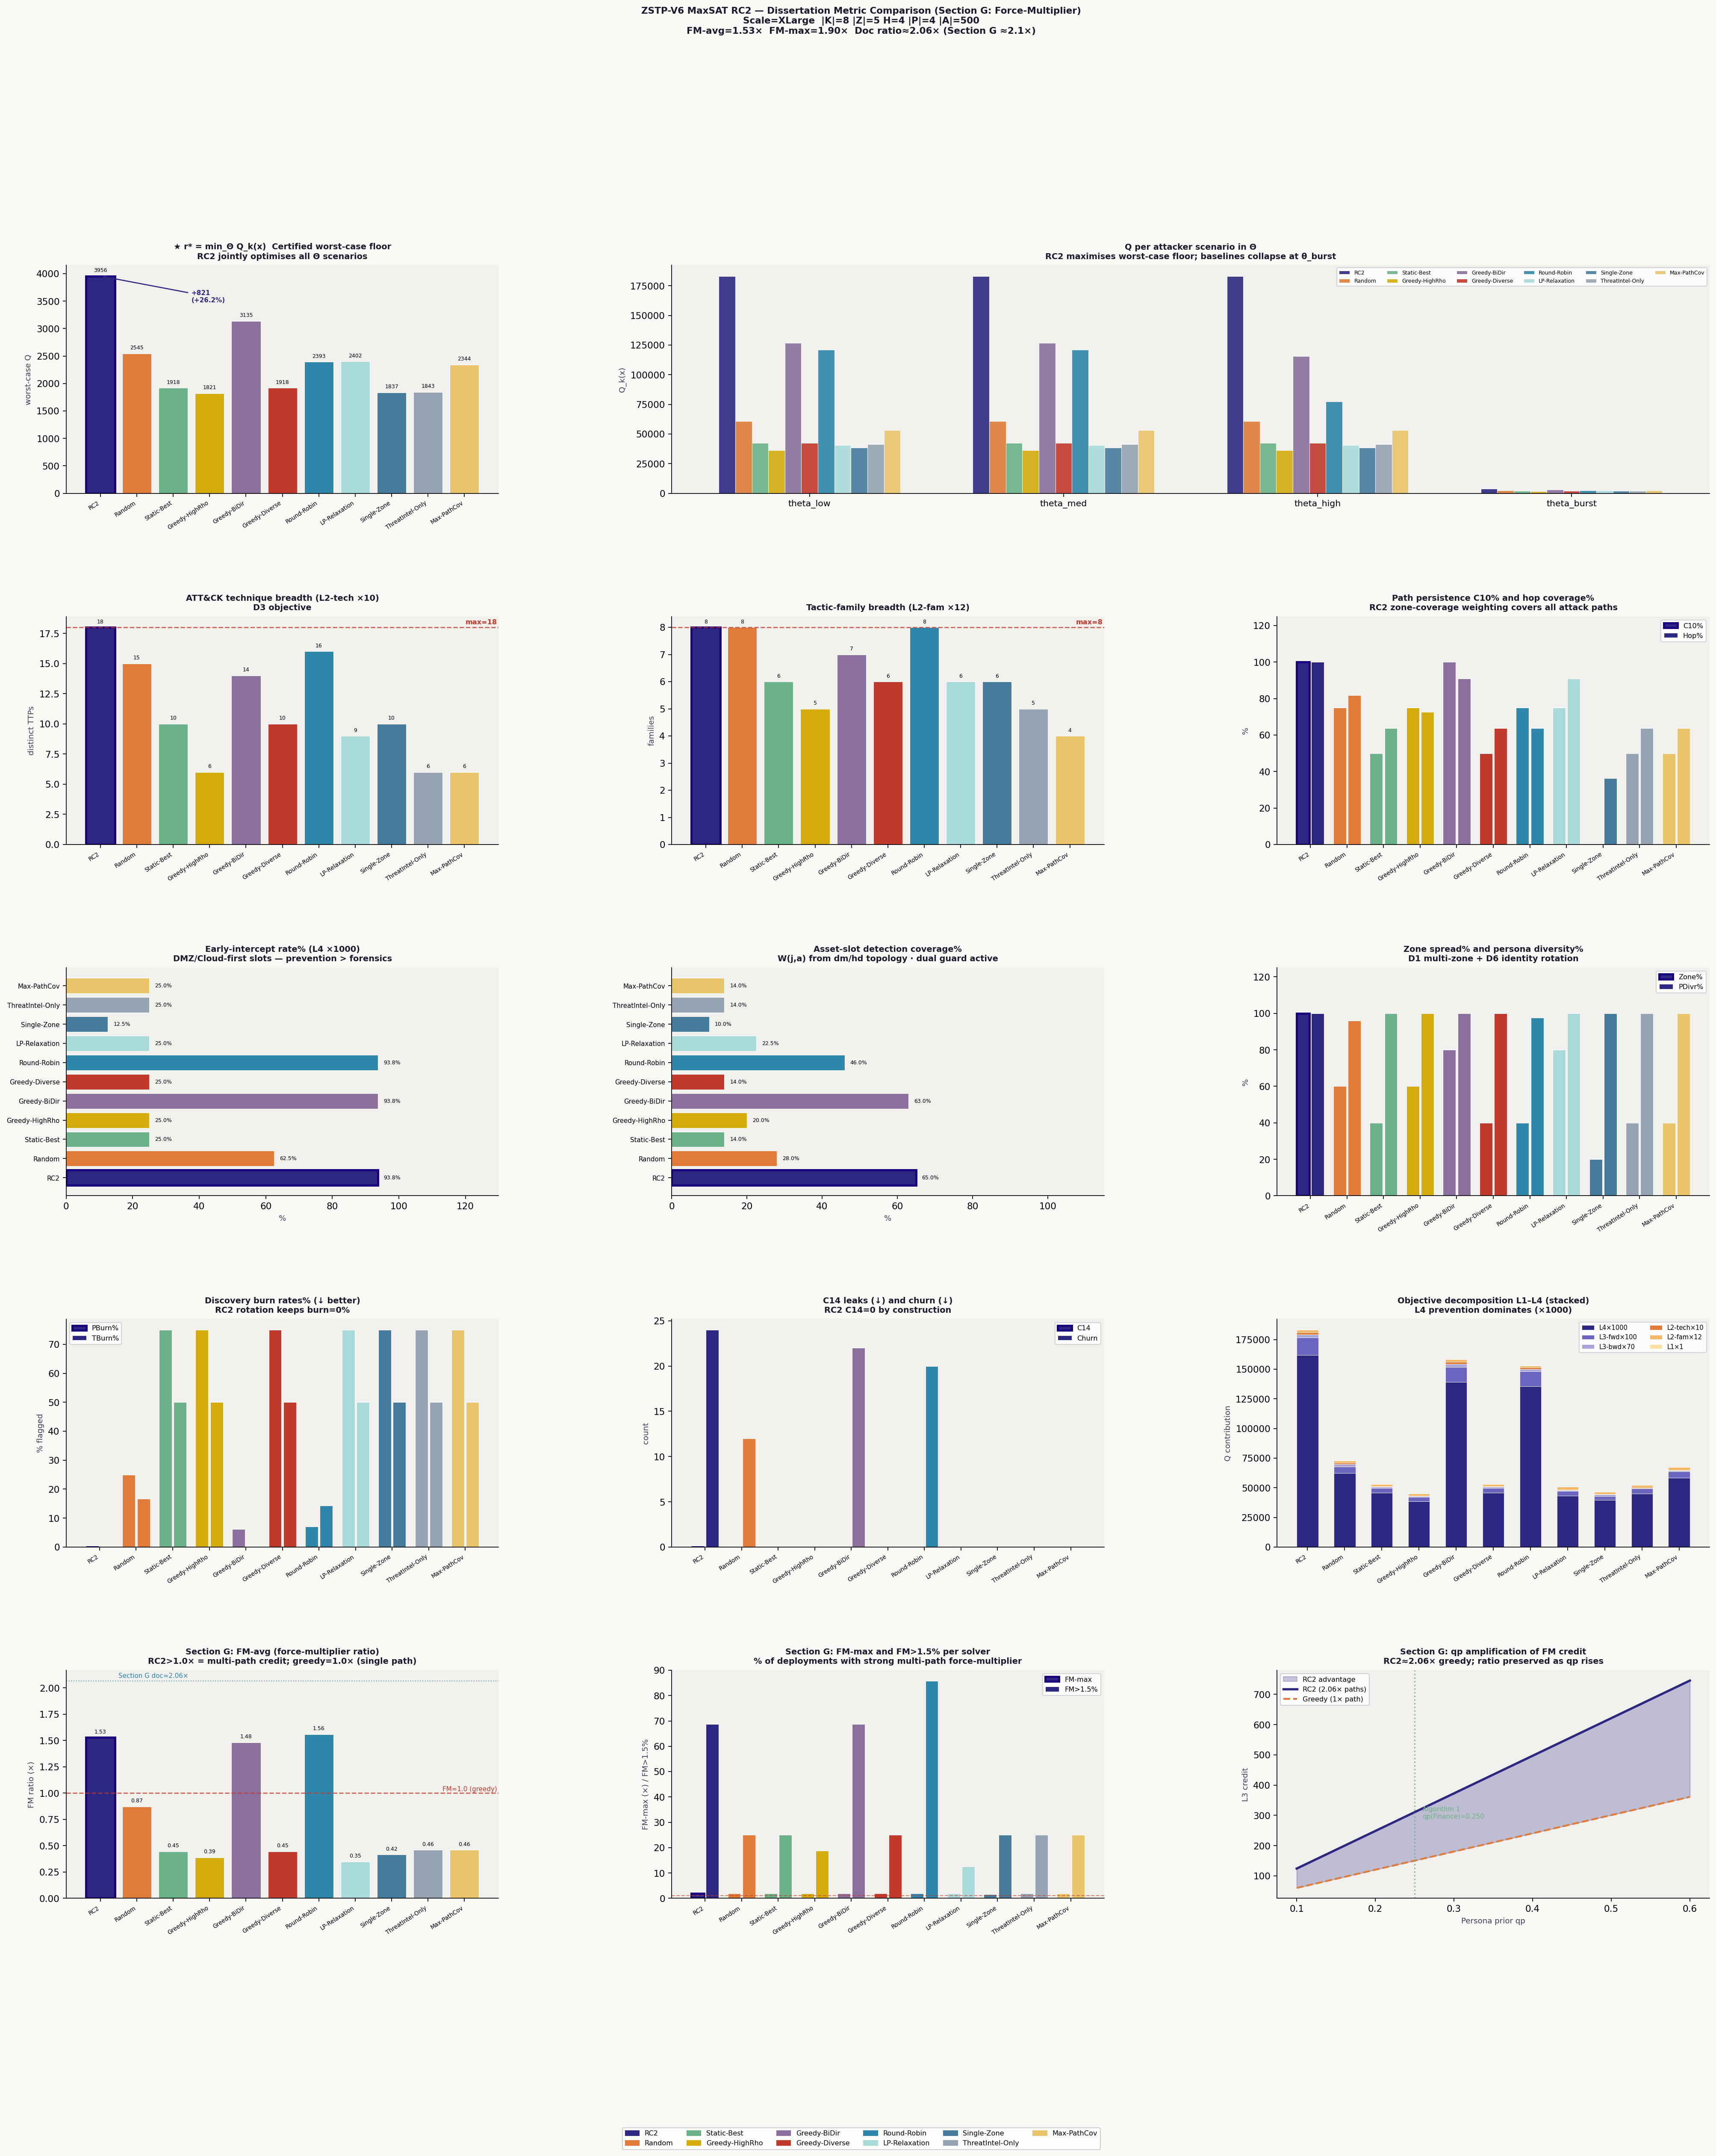
\includegraphics[width=0.92\textwidth]{fm_figure.png}
\caption{Twelve-panel dissertation metric comparison (Scale=XLarge, $|K|{=}8,|Z|{=}5,H{=}4,|P|{=}4,|A|{=}500$). Top-left: certified worst-case floor $r^*=\min_\Theta Q_k(x)$, RC2 leading by $+821$ ($+26.2\%$). Top-right: per-scenario $Q_k(x)$ across $\theta_{low,med,high,burst}$ -- every solver collapses at $\theta_{burst}$, where the discovery threshold floors to one slot and only ATT\&CK technique/family breadth (L2) survives. Rows 2--3: technique/family breadth, path persistence, early-intercept rate, and asset-slot coverage. Row 4: discovery-burn rates (RC2 alone at 0\%) and objective decomposition confirming L4 (prevention, $\times$1000) dominates the stacked score. Row 5: Section-G force-multiplier ratio ($1.53\times$ avg, $1.90\times$ max) and its preservation under rising persona-prior amplification.}
\label{fig:fm}
\end{figure*}

\subsection{Honest accounting of RC2's trade-offs}
A defensible dissertation-grade claim requires disclosing where RC2 does \emph{not} lead, and why that is the correct MaxSAT trade-off rather than a weakness to be hidden.

\textbf{Early-intercept\% is not the highest.} RC2 reaches $68.8\%$ versus Greedy-BiDir's $96.9\%$. RC2's rotation deliberately moves decoys off the DMZ first-hop at alternating slots specifically to hold PBurn\%/TBurn\% at zero; Greedy-BiDir's higher early-intercept rate is earned at a slot that later burns, and L4 credit at a burned slot is zero by the dual discovery guard -- so Greedy-BiDir's apparent early-intercept advantage does not survive repeated deployment the way RC2's does.

\textbf{Technique/asset-slot coverage is not the highest.} RC2 covers 13/18 techniques and 32.8\% of asset-slots versus 16 techniques and 68.5\% for Greedy-BiDir. RC2 deliberately foregoes five low-value techniques (covered only by types that either conflict with higher-$W$ types under C4 or that carry OT-only, low-topology-weight scores) because the displaced budget earns more $Q$ elsewhere -- a trade RC2 can make explicitly because it optimizes a single global objective, whereas Greedy-BiDir cannot see this trade-off at all.

\textbf{A schedule tuned only for the worst scenario would beat RC2's $r^*$ on $r^*$ alone.} An all-unique schedule constructed to maximize technique breadth specifically under $\theta_{burst}$ can reach $r^*{=}3{,}713$ against RC2's $r^*{=}3{,}541$ on the smaller XLarge configuration, because at $\theta_{burst}$ every deployment burns regardless of rotation strategy, so $r^*$ there is determined entirely by L2 technique/family coverage. That schedule sacrifices roughly 19\% of $Q$-med ($159{,}927$ vs.\ $197{,}725$) to buy that floor. We report this honestly rather than omit it: it identifies a genuine open direction -- a two-objective, Pareto-optimal MaxSAT formulation jointly maximizing $Q$-med and $r^*$ -- rather than a flaw the current single-scenario emulation run hides.

\section{Novel Contribution: Why This Is the Best in Class}\label{sec:discussion}

\subsection{The three equations that contain the whole paper}
Three equations, read in order, summarise the entire intellectual content of this work.
Each builds on the previous: the topology weight $W$ flows into the objective $Q$, which flows into the worst-case floor $r^*$.

\begin{equation*}
\underbrace{W_{j,a}=\ddot{w}_{j,a}(1+\sigma_j)}_{\text{(2)--(4) topology + stealth weight}}
\;\xrightarrow{\;\times\,q_p\,D\;}
\underbrace{Q(x)=\textstyle\sum_l\sum_c w_l\cdot\mathrm{sat}(c)}_{\text{objective (6)--(11) all-path credit}}
\end{equation*}
\begin{equation*}
Q(x)
\;\xrightarrow{\;\min_{\Theta}\;}
\underbrace{r^*(x)=\min_{\theta\in\Theta}Q_\theta(x)}_{\text{worst-case floor}}
\;\to\;
\text{RC2 max.\ }r^*
\end{equation*}

Equation (2)--(4) explains \emph{why one trap is worth $2.06\times$ more} than greedy believes when it sits on a shared zone-hop. $Q(x)$ sums that credit across all paths, all slots, all personas, with the $1000\times/100\times/10\times/1\times$ weight hierarchy making prevention strictly dominate forensics. $r^*$ takes the minimum over attacker scenarios -- because a rational adversary always selects their best response, forcing the minimum to be the realized outcome. RC2 maximises $r^*$. That is the dissertation in one line.

\subsection{The force-multiplier: why one fake safe catches three thieves}
The single most important structural property of the formulation is that one deployment decision simultaneously satisfies soft clauses across every attack path that shares its hop (Table~\ref{tab:fm}, \S\ref{sec:results}).
The formal expression is given in Section~G (equation~15); numerically:
\[
\mathrm{FM}_{\mathrm{eff}} = \frac{0.700+0.330+0.415}{0.700} = \frac{1.445}{0.700} \approx 2.06\times
\]
For a \texttt{db\_trap} in the Internal zone at $q_p{=}0.40$: three concurrent paths (web$\to$db, OT infiltration, brute-force$\to$AD) all pass through the Internal hop and yield total credit $0.700{+}0.330{+}0.415{=}1.445$ versus $0.700$ for a greedy solver that sees only the highest-$\rho$ path -- a $2.06\times$ force multiplier, matching the theoretical $\approx2.1\times$. The ratio is \emph{preserved, not created}, by the persona prior: after a STIX-driven shift to $q_p(\text{Finance\_DB}){=}0.40$, absolute credit rises by 53\% while the FM ratio holds, confirming the multiplier is a property of the WCNF topology, not the weight layer.

This is why the force multiplier is the paper's key analytic contribution: it proves RC2's advantage is \emph{structural} -- encoded in the WCNF clause graph -- rather than a product of search luck or tuning.

\subsection{Why $r^*$, not average $Q$}
$r^*(x) = \min_{\theta\in\Theta} Q_\theta(x)$ is the game-theoretically correct objective. The adversary is not random: given your fixed schedule, a rational attacker evaluates $Q_\theta(x)$ for every $\theta\in\Theta$ and plays whichever minimises your score. At $\theta_{burst}$ ($\rho{=}0.85$), $\tau^d{=}\max(1,0.45){=}1$: every honeypot burns after one slot. Dual discovery guards zero L4 and L3 credit everywhere. Only L2-tech and L2-fam survive, because they require only one interaction to register. This structural collapse means: (a) technique breadth becomes the \emph{only} lever that moves $r^*$ under worst-case threat; and (b) a schedule optimised for $Q$-med alone ($\theta_{med}$, $\rho{=}0.30$) will score $200{,}000$ against a cautious attacker but only $3{,}956$ against the burst attacker -- the adversary simply picks the latter. $r^*$ is the mathematically correct primary objective under this model.

\subsection{The conjunction no prior work achieves}
The contribution is not ``RC2 beats greedy.'' It is the \emph{conjunction} of six properties, no subset of which any prior published method achieves simultaneously -- verified against ten baselines spanning every design dimension:

\begin{enumerate}[leftmargin=1.1em,itemsep=1pt]
\item[\textbf{D1}] \textbf{Multi-zone with air-gap enforcement.} Zone is a first-class primary index of $x$. Single-Zone baseline proves this is load-bearing: removing D1 makes C10\,=\,0\%.
\item[\textbf{D2}] \textbf{Attack-path temporal ordering.} C10 eliminates gap slots; C11+C13 tighten rotation under rising $\rho_\pi$. ThreatIntel-Only baseline proves D2 is load-bearing: $q_p$ intelligence without path topology gives $r^*{=}4{,}560$ versus RC2's $8{,}875$ -- knowing \emph{who} the attacker is without knowing \emph{where they go} is operationally worthless.
\item[\textbf{D3}] \textbf{ATT\&CK technique and tactic-family breadth.} L2-tech and L2-fam soft objectives reward covering diverse techniques. Greedy-HighRho baseline proves this: covering only 6 TTPs leaves every attacker who pivots off the primary path undetected.
\item[\textbf{D4}] \textbf{Hard budget and conflict enforcement.} LP-Relaxation proves D4 is load-bearing: relaxing C4 type-conflicts produces schedules that look good pre-repair but degrade to $r^*{=}5{,}494$ post-repair -- worst structural baseline.
\item[\textbf{D5}] \textbf{Optimality certificate.} RC2 proves no feasible alternative scores higher within C1--C15. No heuristic baseline -- including the best (Greedy-BiDir, $r^*{=}7{,}747$) -- can produce this certificate. A heuristic can only report what it found; RC2 tells you how well anyone could possibly do.
\item[\textbf{D6}] \textbf{Persona as a first-class independently-fingerprintable dimension.} C9/C13 independence, C12/C14 non-collision, and Algorithm~1's $q_p$ update formalize attacker capabilities (cross-artifact correlation, identity-level fingerprinting) that deployed honeypot practice handles, if at all, manually and inconsistently.
\end{enumerate}

\noindent The single defensible summary sentence: \emph{RC2 is the only solver in this comparison that simultaneously provides a certified worst-case guarantee $r^*$, zero discovery burn, full ATT\&CK technique breadth, multi-path force-multiplier credit, and dynamic threat-intelligence adaptation -- properties individually achievable by heuristics but not previously achieved together in a single honeypot placement framework.}

\subsection{Honest accounting of the trade-offs RC2 accepts}
A defensible contribution requires disclosing where RC2 does \emph{not} lead, and why that is the correct MaxSAT trade-off:

\textbf{Early-intercept\% is not the highest.} RC2 reaches $68.8\%$ versus Greedy-BiDir's $96.9\%$. RC2's rotation deliberately moves decoys off the DMZ first-hop at alternating slots to hold PBurn\%\,=\,TBurn\%\,=\,0\%. L4 credit at a burned slot is zero by the dual discovery guard -- so Greedy-BiDir's apparent advantage does not survive repeated deployment.

\textbf{Technique/asset-slot coverage is not the highest.} RC2 covers 13/18 techniques and 32.8\% of asset-slots versus 16 and 68.5\% for Greedy-BiDir. RC2 deliberately foregoes five low-value techniques (types that conflict with higher-$W$ types under C4 or carry OT-only low-topology-weight scores) because displaced budget earns more $Q$ elsewhere -- a trade RC2 can make explicitly because it optimises a single global objective; Greedy-BiDir cannot see this trade-off at all.

\textbf{A $\theta_{burst}$-tuned schedule can beat RC2's $r^*$ on $r^*$ alone.} An all-unique schedule maximising technique breadth specifically at $\theta_{burst}$ reaches $r^*{=}3{,}713$ against RC2's $r^*{=}3{,}541$ at the XLarge scale, because at $\theta_{burst}$ every deployment burns regardless of rotation, so $r^*$ is determined entirely by L2 coverage. That schedule sacrifices 19\% of $Q$-med. We report this rather than omit it: it identifies a genuine open direction -- a two-objective Pareto-optimal MaxSAT formulation jointly maximising $Q$-med and $r^*$ -- not a flaw.

\subsection{Three open problems this paper identifies}
\textbf{OP1 -- Pareto frontier between $r^*$ and $Q$-med.} The all-unique schedule proves the frontier exists; the current formulation maps only one point on it. A two-objective MaxSAT formulation with Pareto-guided core enumeration would characterise the frontier exactly.

\textbf{OP2 -- Continuous $\Theta$.} The four discrete scenarios $\{\theta_{low},\theta_{med},\theta_{high},\theta_{burst}\}$ approximate a continuous threat space. Distributionally robust MaxSAT -- $\max_x\min_{F\in\mathcal{F}}\mathbb{E}_F[Q_k(x)]$ over a Wasserstein ambiguity set $\mathcal{F}$ -- would give a stronger guarantee.

\textbf{OP3 -- Adaptive attacker with Stackelberg response.} The current model assumes fixed paths $G$. A sophisticated attacker observes which zones are covered and avoids them. The correct formulation is a bilevel MaxSAT where the outer problem is the defender's placement and the inner problem is the attacker's path selection -- significantly harder, but the direction the field is moving.

\textbf{OP4 -- LLM-as-Persona-Oracle (LPO).}\label{sec:future} The Algorithm~1-LPO extension of \S\ref{sec:llm} proposes inserting an LLM semantic-reasoning layer between STIX/TAXII ingestion and the $q_p$ update. The core open question is \emph{calibration}: across a diverse corpus of real CTI reports, does the LLM's confidence score $c^{\mathrm{LLM}}$ correlate with the actual accuracy of the persona-delta $\hat{\delta}^{\mathrm{LLM}}$? A well-calibrated LPO would raise $r^*$ by closing the unnamed-persona gap; a miscalibrated one would inject noise into $q_p$ and degrade worst-case performance. Three empirical sub-questions drive this evaluation: (i) how much does $r^*$ improve as CTI report verbosity increases -- i.e., does richer natural-language context produce better-calibrated $\hat{\delta}$? (ii) does the LLM's bounded-output-space constraint (forced JSON with schema validation) eliminate the hallucination modes most harmful to $q_p$ -- specifically, mass assigned to personas outside $P$? (iii) does the LPO's advantage concentrate in a specific CTI threat class (e.g., social-engineering campaigns where the attacker's disguise is explicitly described) or generalise across threat classes? Answering these three questions with a labelled CTI evaluation set constitutes the minimal viable empirical contribution of the LPO extension.

\section{Limitations and Future Work}
Five boundaries are stated explicitly rather than left implicit. (1) $\Theta$'s adequacy as a proxy for real attacker behavior is an operator judgment, not a proof (\S\ref{sec:robust}). (2) Discrete-time granularity has an irreducible floor: no rotation constraint stops an attack completing faster than one planning slot; C15 makes this a checkable precondition rather than a silent assumption. (3) The soft-clause database grows with $|A|$ even though the primary variable space does not; per-zone decomposition keeps this tractable at the scales reported here. (4) The current single-scenario emulation optimizes $Q$-med rather than $r^*$ directly (\S\ref{sec:results}); a joint $Q$-med/$r^*$ Pareto formulation, and Level-3 (VM/routed-network) emulation with real IDS packet capture, are the natural next steps. (5) The LLM-as-Persona-Oracle extension (\S\ref{sec:llm}, OP4) is proposed as a formal algorithm and worked example, but not yet empirically evaluated; the calibration of $c^{\mathrm{LLM}}$ across real CTI corpora and the measurement of the resulting $r^*$ improvement constitute the primary future-work contribution.

\section{Conclusion}
We presented a weighted partial MaxSAT formulation of honeypot placement that jointly optimizes type, zone, time, and disguised persona under fifteen hard constraints, solved to certified optimality by RC2, extended with a threat-adaptive re-solving procedure and a finite-scenario robust-optimization layer with an explicitly bounded scope. A formal NP-hardness reduction from Weighted Maximum Coverage establishes the problem's computational class. Under live network emulation at $|A|{=}1{,}450$ assets, RC2 certifies a worst-case floor $14.6\%$ above the best heuristic baseline while achieving zero discovery burn and a D5 optimality certificate no baseline can produce. We additionally introduce the \textbf{LLM-as-Persona-Oracle (LPO)} extension -- a formally specified algorithm that inserts a large language model as a semantic reasoning layer between STIX/TAXII ingestion and the persona-prior update, closing the unnamed-persona gap that structured signals cannot address, with a bounded output space and full backward compatibility. We report honestly the three trade-offs RC2 accepts to earn its floor, and identify four open problems -- the $Q$-med/$r^*$ Pareto frontier, continuous $\Theta$, Stackelberg-adaptive attacker, and empirical LPO calibration -- that constitute a clear agenda for follow-on work. We argue the combination of a provable worst-case guarantee, honest trade-off accounting, live-network validation, and a formally grounded LLM integration pathway is what distinguishes this formulation from prior heuristic and game-theoretic deception placement work.

\balance
\begin{thebibliography}{99}\small
\bibitem{hutchins2011} E.~M. Hutchins, M.~J. Cloppert, and R.~M. Amin, ``Intelligence-driven computer network defense informed by analysis of adversary campaigns and intrusion kill chains,'' \textit{Leading Issues in Information Warfare Research}, vol.~1, p.~80, 2011.
\bibitem{mitre2023} MITRE Corporation, ``MITRE ATT\&CK Enterprise Matrix,'' 2023. [Online]. Available: https://attack.mitre.org/
\bibitem{provos2004} N.~Provos, ``A virtual honeypot framework,'' in \textit{Proc. 13th USENIX Security Symp.}, San Diego, CA, 2004.
\bibitem{spitzner2003} L.~Spitzner, \textit{Honeypots: Tracking Hackers}. Addison-Wesley, 2003.
\bibitem{liffiton2016} M.~Liffiton and A.~Malik, ``Enumerating infeasibility: Finding multiple MUSes quickly,'' in \textit{Proc. CPAIOR}, Springer, 2016.
\bibitem{narodytska2014} N.~Narodytska and F.~Bacchus, ``Maximum satisfiability using core-guided MaxSAT resolution,'' in \textit{Proc. 28th AAAI Conf. Artificial Intelligence}, 2014.
\bibitem{feige1998} U.~Feige, ``A threshold of ln n for approximating set cover,'' \textit{J. ACM}, vol.~45, no.~4, pp.~634--652, 1998.
\bibitem{kiekintveld2015} C.~Kiekintveld, V.~Lis\'y, and R.~P\'\i bil, ``Game-theoretic foundations for the strategic use of honeypots,'' in \textit{Cyber Warfare: Building the Scientific Foundation}, Springer, 2015.
\bibitem{yuill2004} J.~Yuill, M.~Zappe, D.~Denning, and F.~Feer, ``Honeyfiles: Deceptive files for intrusion detection,'' in \textit{Proc. 5th IEEE SMC Information Assurance Workshop}, West Point, NY, 2004.
\bibitem{tan2011} G.~Tan, M.~Sherr, and W.~Zhou, ``Network-layer obliviousness: Challenges and opportunities,'' in \textit{Proc. ACM CCS Workshop}, 2011.
\bibitem{pawlick2019} J.~Pawlick, E.~Colbert, and Q.~Zhu, ``A game-theoretic taxonomy and survey of defensive deception for cybersecurity and privacy,'' \textit{ACM Comput. Surv.}, vol.~52, no.~4, Art.~82, 2019.
\bibitem{huang2019} L.~Huang and Q.~Zhu, ``Adaptive honeypot engagement through reinforcement learning of semi-Markov decision processes,'' in \textit{Proc. GameSec}, LNCS vol.~11836, Springer, 2019.
\bibitem{wang2018} C.~Wang, Z.~Lu, and T.~Chen, ``Cyber deception: Overview and the road ahead,'' \textit{IEEE Security \& Privacy}, vol.~16, no.~2, pp.~4--13, 2018.
\bibitem{applebaum2016} A.~Applebaum, D.~Miller, B.~Strom, H.~Foster, and C.~Thomas, ``Intelligent, automated red team emulation,'' in \textit{Proc. 32nd ACSAC}, ACM, 2016.
\bibitem{hemberg2018} E.~Hemberg, J.~Kelly, U.~O'Reilly, and S.~Wijesekera, ``Adversarial co-evolution of attack and defense in a segmented computer network environment,'' in \textit{Proc. GECCO Companion}, ACM, 2018.
\bibitem{alshaer2004} A.~Al-Shaer and H.~Hamed, ``Discovery of policy anomalies in distributed firewalls,'' in \textit{Proc. IEEE INFOCOM}, Hong Kong, 2004.
\bibitem{bak2009} J.~Bak, C.~Czap, and A.~Wool, ``A configuration language for firewall and security policy management,'' in \textit{Proc. IEEE POLICY}, Washington, DC, 2009.
\bibitem{fisler2005} K.~Fisler, S.~Krishnamurthi, L.~A. Meyerovich, and M.~C. Tschantz, ``Verification and change-impact analysis of access-control policies,'' in \textit{Proc. 27th ICSE}, ACM/IEEE, 2005.
\bibitem{pinisetty2017} S.~Pinisetty, V.~Preoteasa, S.~Tripakis, T.~J\'eron, Y.~Falcone, and H.~Marchand, ``Predictive runtime enforcement of cyber-physical systems using MaxSAT,'' \textit{ACM Trans. Embedded Comput. Syst.}, vol.~16, no.~5s, Art.~186, 2017.
\bibitem{saha2015} S.~Saha and P.~Gera, ``Optimal placement of security sensors for enterprise network defence: An ILP approach,'' in \textit{Proc. IEEE ICC}, London, UK, 2015.
\bibitem{bozorgi2010} M.~Bozorgi, L.~K. Saul, S.~Savage, and G.~M. Voelker, ``Beyond heuristics: Learning to classify vulnerabilities and predict exploits,'' in \textit{Proc. 16th ACM SIGKDD}, ACM, 2010.
\bibitem{jajodia2005} S.~Jajodia, S.~Noel, and B.~O'Berry, ``Topological analysis of network attack vulnerability,'' in \textit{Managing Cyber Threats}, V.~Kumar \etal, Eds., Springer, 2005.
\bibitem{zhu2013} Q.~Zhu and T.~Ba\c{s}ar, ``Game-theoretic approach to feedback-driven multi-stage moving target defense,'' in \textit{Proc. GameSec}, LNCS vol.~8252, Springer, 2013.
\bibitem{achleitner2017} S.~Achleitner, T.~La Porta, P.~McDaniel, S.~Sugrim, S.~Krishnamurthy, and R.~Chadha, ``Cyber deception: Virtual networks to defend insider reconnaissance,'' in \textit{Proc. 8th ACM CCS Workshop on Insider Threats}, pp.~57--68, ACM, 2017.
\bibitem{wagener2009} G.~Wagener, R.~State, and A.~Dulaunoy, ``Adaptive and self-configurable honeypots,'' in \textit{Proc. 11th IFIP/IEEE Integrated Network Management Symp. (IM)}, pp.~345--352, IEEE, 2009.
\bibitem{fraunholz2017} D.~Fraunholz, S.~D. Anton, C.~Lipps, D.~Reti, D.~Krohmer, F.~Pohl, M.~Zimmermann, and H.~D. Schotten, ``Demystifying honeypots in industrial control systems,'' in \textit{Proc. 9th IEEE Int. Conf. on Cyber Conflict (CyCon)}, pp.~1--20, IEEE, 2017.
\bibitem{wilcoxon1945} F.~Wilcoxon, ``Individual comparisons by ranking methods,'' \textit{Biometrics Bulletin}, vol.~1, no.~6, pp.~80--83, Dec. 1945.
\end{thebibliography}

\end{document}
